
\documentclass[sigconf]{acmart}

%%
%% \BibTeX command to typeset BibTeX logo in the docs
\AtBeginDocument{%
  \providecommand\BibTeX{{%
    \normalfont B\kern-0.5em{\scshape i\kern-0.25em b}\kern-0.8em\TeX}}}

%% Rights management information.  This information is sent to you
%% when you complete the rights form.  These commands have SAMPLE
%% values in them; it is your responsibility as an author to replace
%% the commands and values with those provided to you when you
%% complete the rights form.
\setcopyright{acmcopyright}
\copyrightyear{2019}
\acmYear{2019}
\acmDOI{}

%% These commands are for a PROCEEDINGS abstract or paper.
%\acmConference[Woodstock '18]{Woodstock '18: ACM Symposium on Neural
%  Gaze Detection}{June 03--05, 2018}{Woodstock, NY}
%\acmBooktitle{Woodstock '18: ACM Symposium on Neural Gaze Detection,
%  June 03--05, 2018, Woodstock, NY}
%\acmPrice{15.00}
%\acmISBN{978-1-4503-9999-9/18/06}


\begin{document}

\title{Comparison of Two Proactive Self-adaptation Methods: PLA and CobRA}


\author{Ben Trovato}
\authornote{Both authors contributed equally to this research.}
\email{trovato@corporation.com}
\orcid{1234-5678-9012}
\author{G.K.M. Tobin}
\authornotemark[1]
\email{webmaster@marysville-ohio.com}
\affiliation{%
  \institution{Institute for Clarity in Documentation}
  \streetaddress{P.O. Box 1212}
  \city{Dublin}
  \state{Ohio}
  \postcode{43017-6221}
}

\author{}
\affiliation{%
  \institution{The Th{\o}rv{\"a}ld Group}
  \streetaddress{1 Th{\o}rv{\"a}ld Circle}
  \city{Hekla}
  \country{Iceland}}
\email{larst@affiliation.org}

\author{}
\affiliation{%
  \institution{Inria Paris-Rocquencourt}
  \city{Rocquencourt}
  \country{France}
}
%\begin{verbatim}
%\bibliographystyle{ACM-Reference-Format}
%\bibliography{acmart}
%\end{verbatim}

\begin{abstract}
Software-intensive systems tend to face more and more uncertainties in running environment, which are difficult to  engineer and expensive to consider at design time. Therefore, software systems need to have ability of self-adaptation, to monitor the change of uncertainties and adjust itself dynamically to keep approaching the target. As we consider which methods we should choose to use, we weigh their engineering costs and resulting effects. Currently, there are most advanced two proactive adaptive methods, PLA  and CobRA, both adopting ideas from MPC. They spend different efforts on modeling and achieve different effects. We hope to explore which method can achieve better adaptive effect with less effort under different application scenarios. In this paper, we compare PLA and CobRA applied to a benchmark system for web and cloud application performance, RUBiS. Both of the two methods require the environment to change slowly and regularly. PLA needs more efforts on engineering whereas MPC can tolerate more uncertainties due to its feedback mechanism. In view of their advantages and disadvantages, We look at ways to design better.
\end{abstract}

\begin{CCSXML}
	<ccs2012>
	<concept>
	<concept_id>10011007.10010940.10010971</concept_id>
	<concept_desc>Software and its engineering~Software system structures</concept_desc>
	<concept_significance>300</concept_significance>
	</concept>
	</ccs2012>
\end{CCSXML}

\ccsdesc[300]{Software and its engineering~Software system structures}

\keywords{self-adaptation, PLA, CobRA, model predictive control}

\maketitle

\section{Introduction}
Why do software systems need  capabilities of self-adaptation?
The main reason is that software-intensive systems face a lot of uncertain factors while running, such as the change of running environment and the change of requirements. While in the construction stage of software systems, considering all those changes is not easy and needs high cost. However, due to some properties of the software system, we can design an adaptive mechanism to tolerate these uncertain changes, which is the fundamental purpose of self-adaptation. The main difference between traditional software engineering and self-adaptation software engineering is that, in traditional software, we will anticipate changes that the software system will face in the future and give the response to them. On the contrary, for self-adaptation, we do not need to design as carefully as possible the solution to all changes that maybe happen, we just need to know some feature of the system, then we can design an adaptation controller to handle these changes according to these features.
Software self-adaptation is that software can monitor uncertainties during running, then make adaptive tactics to adjust itself to response to these changes in order to maximize its goal.

However traditional software self-adaptation are reactive, they only make adaptive tactices after changes happened, do not predict what will happen in the future. On the contrary, proactive self-adaptation can predict what will happen in the future, to make tactices ahead of time. Proactive self-adaptation also bases on MAPE-K loop control\cite{mape}, consisting monitor, analyze, plan, and execute modules sharing a whole knowledge. We are more concerned with the implementation of analyze and plan module.

Currently, there are two advanced methods of proactive self-adaptation,PLA and CobRA, both apply ideas from MPC(model predictive control). PLA is based on traditional software engineering. It constructs the system to a MDP model and predicts future environment to model the environment as a DTMC. It explicitly constructs the requirements of the system to a revenue  function. Then we can use probablistic model checkers, such as PRISM to analyse the whole MDP model to get control tactics. The main feature of PLA is that it is an open-loop method. Its effectiveness depends largely on the accuracy of the model. Thus it needs a lot of effort to build the model of system and environment as accurately as possible. CobRA uses more ideas from control theory. It constructs the system to a simple liner model. Rather than predicting the future environment, it regards the variation of enviornment as disturbance of the system, and use Kalman Filter to reflect the disturbance on the state of the system. CobRA is a feedback method and need fewer effort to build model of the system. However, feedback methods have weaknesses such as they are usually one step behind the real situation.

When we are considering which method to choose, there are some facts that we need to weigh. The most important one is whether the method can handle our problem and achieve the goal of object system. Because when we model the system, we are simplifying the system, thus inevitably there will have errors between the model and the real system. Unlike in the physical world, which can be modeled by exact mathematical equations, software systems are always more complex to model. Althogh it seems that MDP is more accurate than linear model, but it also exist errors and need more efforts while building. CobRA is not much precise, but it has many theory of guarantees of stability. If we can achieve similar results, obviously we want to use method that needs fewer effort.

Gabriel A. Moreno compared the two methods both in terms of development complexity and run-time performance. While the two approaches perform comparably in general, their run-time behavior can be significantly different, both in terms of resource utilization and the ways in which they attempt to maximize performance. We can see that both of them can get fine results after elaborate adjustment of feedback parameters. But we want to compare the two methods at the methodological level rather than on a certain system. We carry out more detailed experiments and get more conclusions.

In this paper, we compare the two methods on the methodological level. First we analyze from the design ideas of the two methods to find their strengths and weaknesses. Then we use experiments to show more concrete results. We illustrate our comparison on the Rice University Bidding System (RUBiS), an open-source application widely employed as a benchmark in cloud computing and for evaluation of self-adaptive solutions. To enable a fair comparison of the two approaches, we ran our experiments in a simulation of RUBiS. In that way, we were able to avoid uncontrolled effects that could alter the results of experiments with the real system (e.g., background processes, network delays).

From the perspective of soft engineering, we want to find what effort is required for the two methods respectively, and then from the perspective of effect, what effect did the two methods have respectively. The results of our study show that both of the two methods apply MPC ideas, they have the same goal, but have different effects. CobRA is more tolerant of uncertainty, such as uncertain environment and model error. If there are non-negligible in prediction and modeling, PLA may achieve poor effect and need more effort in design and run-time phase. We find that PLA works a lot depends on feedback. In the future work, we want to explore the effect of feedback-PLA, in which case we combine CobRA with the prediction in PLA.

In the remainder of the paper, Section II presents the details of the adaptation scenario employed for our comparative study. Section III provides a summary of the main ideas behind model predictive control, as well as an overview of CobRA and PLA. Next, Section IV details our comparison and discusses results. Section V describes related work. Finally, Section VI presents conclusions and future research directions. 

\section{adaptation senario}

We illustrate our comparison on the Rice University Bidding System (RUBiS)\cite{rubis}, an open-source application widely employed as a benchmark in cloud computing [11]–[13] and for evaluation of self-adaptive solutions [7], [14]. 
To enable replicating experiments with the same conditions under control for the two approaches, avoiding unexpected fluctuation and uncertainties during real systems running, we ran our experiments on a simulated system of RUBiS, which is named SWIM.

RUBiS system consists of a load-balancer, a web server tier and a database tier. Clients use browsers to send requests to the server. Load balancer distributes requests among servers following a round-robin policy. Servers access the database to obtain the data required to render the dynamic content of the page.
Figure \ref{fig:rubis} shows the architecture of RUBiS system. 
\begin{figure}[h]
	\centering
	
\includegraphics[width=\linewidth]{rubis}
	\caption{Architecture of RUBiS}
\end{figure}

\begin{itemize}
	\item {\verb|Uncertainties|}:
	
	The main uncertainties of rubis system, which is need to sovled by the adaptation controller, are three types:
	\begin{enumerate}
		\item The uncertainty from environment. For RUBiS system, the only relevant property of the operating environment that we consider in our adaptation scenario is the  prescribed by the workload induced on the system. If the request arrival rate increases suddenly, the system need more resource to handle them.
		\item The uncertainty from the latency of adding a server. For RUBiS system, there is a period time that before a new server can start working. We call it \textit{latency} of adding servers. 
		\item The uncertainty of how long it needs to process a request. That is the service time in RUBiS system.
	\end{enumerate}
	\item {\verb|Tactics|}: 
	For RUBiS system, the main uncertainty that self-adaptation want to handle is the uncertain environment. RUBiS system can execute two types of tactic to adjust itself to deal with uncertainties:
	\begin{itemize}
		\item Add/remove server. There is a delay in adding a server, which we call it latency, whereas removing a server can be consider as no latency, because the latency for removing a server is negligible.
		\item Increase/decrease dimmer value. RUBiS system follows the brownout paradigm\cite{brownout}, which can response to a request includes mandatory content and optional content. The dimmer parameter indicates the proportion of a request including optional content.
	\end{itemize}
	\item {\verb|Utility|}:
	The goal of the target system can be described as two functional and three non-functional requirements. Functional requirements are tasks of the system, whereas we capture non-functional requirements formally in a utility function that enables us to quantify the quality of their satisfaction. The utility function is modeled as follows:
	\begin{equation}
	\begin{aligned}
	U_{\tau}=\left\{
	\begin{array}{rcl}
	U_{R}+U_{C} & & { r\leq T\wedge U_{R}=U_{R}^{*}} \\
	U_{R} & & {r\leq T\wedge U_{R}<U_{R}^{*}}\\
	\tau min(0,\alpha-\kappa)R_{O} & & {r>T}\\
	\end{array} \right.
	\end{aligned}
	\end{equation}
	\begin{itemize}
		\item utility associated with \textit{cost }per time interval:
		\begin{equation}
		U_{C}=\tau \cdot c\cdot (s^{*}-s)
		\end{equation}
		\item utility associated with revenue per time interval:
		\begin{equation}
		U_{R}=\tau \cdot \alpha \cdot (d\cdot R_{O}+(1-d)\cdot R_{M})
		\end{equation}
		where $\tau$ is the length of the interval, $\alpha$ is the average request rate, and \textit{d} is dimmer value. $R_{M}$ and $R_{O}$ are the rewards for serving a request with mandatory and optional content,respectively.
	\end{itemize}
	The most important requirement is keeping the response time $r$ below the threshold $T$. The second one is the target system shall provide high quality of service, which is described by dimmer value $d$. The third one is that the target system shall use little number of servers $s$ to operate under low cost. The whole goal is to get higher revenue while generate lower cost.
\end{itemize}


\section{Two proactive self-adaptaion methods: PLA and CobRA}
Both of the two approach are based on MPC idea. That is, 1) use models to predict behavior of system, 2) adopt idea of receding horizon. To achieve proactive features, both of them consider a adaptation horizon, which is some periods in the future. There are still considerable differences between them. We will discuss their similarities and differences in detail.
\begin{itemize}
	\item {\verb|Adaptation uncertainties|}:
	There are two kinds of uncertainties faced by self-adaptation controller. One is the uncertainty to be solved by the adaptive system, which is the external uncertainty. For RUBiS system, it includes the arriving rate of requests, the delay of how long it takes to start a server, and how long it takes to process a request, etc. The other type is the uncertainties faced in the design of controller. One is that there will be errors between the actual system and the model, as well as in the PLA's environmental prediction and data measurement.
	The solution of the first kind of uncertain reflects the control effect of the adaptive method itself.
	Tolerance for the second type of uncertainty reflects the properties of the controller, such as stability, which can be measured by SASO properties\cite{saso}.
	The second type of uncertainty will seriously affect the realization of the the non-functional requirements . In order to ensure the completion of their control goals, excellent controllers need to have the ability to tolerance uncertainties.
	\item {\verb|Adaptation goal|}:
	The goal of adaption controller is to decide how to adapt to maximize the utility the system will accrue over the look-ahead horizon, with the monitoring, analysis, planning and executing part, dealing with the influence of uncertainties. And we expect the controller performance is robust, having the ability of resisting disturbance.
\end{itemize}
\subsection{PLA}
The key idea of PLA is to let the adaptation decision underspecified through nondeterminismuse and construct a formal model of the adaptive system, then have the model checker resolve the nondeterministic choices to achieve the accumulated utility over the horizon is maximized. The adaptation decision is optimal over the decision horizon, and takes into account the inherent uncertainty of the environment predictions needed for looking ahead.

For PLA, decisions are made not only based on historical circumstances and current measurements, but also on the predicted future. We discretizes the execution of adaptation decison in periods of $\tau$, and the system behavior in the adaptation horizon is predicted by modeling the system into a MDP, which uses state changes to express the execution of adaptation tactics.

The environment can be modeled as a DTMC model in which the random variable representing the state of the environment has one change at each evaluation period $\tau$. PLA uses an autoregresive (AR) time series predictor to predict future environment, such as RPS toolkit, which requires that the changes of environment should be predictable and regular. There will be an error in the estimation, the predictor can provide the variance of the estimation. PLA use the Extended Pearson-Tukey (EP-T) threepoint approximation to construct probability trees for decision making. As shown in figure\ref{fig:envtree}, the root $e_{0}$ of the tree is currunt environment, and $e_{1}$ is the estimation distribution of environment in next period with probabilities 0.185, 0.630, and 0.185, respectively.
\begin{figure}[h]
	\centering
	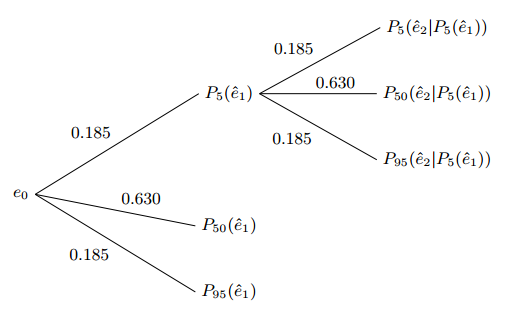
\includegraphics[width=\linewidth]{envtree}
	\caption{Probability Tree of Environment}
\end{figure}

Unfortunately, there will be large errors in the prediction of future environment. In addition, sudden fluctuations cannot be predicted, which will have a great impact on decision-making. This will be analyzed in detail later. Finally, the system and environment are built into a whole MDP model, and the goals of the system are constructed into the form of utiity function. 
For RUBiS system, the models of the system and environment are stored in \textit{knowledge}. At every beginning of adaptation period, monitor gets measurements from the system and then update the models. 

We can use a probability model detector to analyze the model, verify the attributes, exhaust all paths and find a strategy to maximize the revenue function. 
We use LPS queuing theory model to calculate the response time of the system.
In design time, PLA need plenty of effort to build an accurate model of the environment and the target system. It is a feed-forward method, thus the result largely depend on modeling.

\subsection{CobRA}
CobRA adopts more ideas of control theory.
The non-functional requirements of RUBiS system are captured by the softgoals: High Performance, Low Cost, and High Optional Content Availability.
CobRA refers to adaptation goals as \textit{indicators}, for RUBiS system, they are: \textit{r} for average response time of requests, \textit{s} for number of servers and \textit{d} for dimmer value, and constitute the system's output. The parameters of the system that can be tuned in order to fulfil its goals are called \textit{control parameters}. For RUBiS system, \textit{control parameters} are the number of servers \textit{s} and the dimmer value \textit{d}, which constitute the system's input. As well as PLA, CobRA discretizes the execution timeline in adaptation periods of $\tau$, and solves the adaptation decision problem at the start of every period.

CobRA abstracts the relationship between the input and output of the system into a simple linear model. The model represents affects of control parameters to indicators over time. We can use a discrete-time linear dynamic model to describe the system behavior at the k-th decision period.

\begin{equation}
\left\{
\begin{array}{rcl}
x(k+1)=A\cdot x(k)+B\cdot u(k)\\
y(k)=C\cdot x(k)+D\cdot a(k)\\
\end{array} \right.
\end{equation}
where $x$ is the state of the system, $u$ is the set of control parameters, $y$ is the set of indicators and $a(k)$ is the average arrival rate of requests at the k-th decision period.

For the uncertain environment, CobRA does not predict future environment, instead, it treats the environment as disturbance to the system. In our scenario, the environment is uncertain arrival rate of requests \textit{a}, that is used as a feedforward signal. The effect of environment's uncertainty is reflected by Kalman Filter on the system's states.

CobRA is requirement-based, fot RUBiS system, the system's goal can be described as three output variables: the number of servers \textit{s}, the dimmer value \textit{d}, and the average response time of requests \textit{r}.
The goal of the system is that each indicator should be close to its target value, and the goal of the system is designed into the form of cost-function. CobRA make decisions by modifying the value of the control variables.
\begin{equation}
\begin{aligned}
&J_{k}=\sum_{i=1}^H [y_{k+i}^o -y_{k+i}]^TQ_{i}[y_{k+i}^o -y_{k+i}] \\
&+[\Delta u_{k+i-1}]^T P_{i}[\Delta u_{k+i-1}]
\end{aligned}
\end{equation}
where $Q_{i}$ and $P_{i}$ are symmetric positive semi-definite wetghting matrics. $Q_i$ means that when not all the goals can be achieved, the controller will prefer the satisfaction of the goals with high weights. $P_i$ means that the controller want to change the control parameters frequently with smaller weight. $y_{k+i}^o$ are setpoints of indicator i, which means the goal value of this indicator. 

The optimization problem can be definited as follows:
\begin{equation}
\begin{aligned}
&minimize_{\Delta u_{k+i-1}}\qquad J_t \\
&subject\quad to \qquad u_{min}\leq u_{k+i-1}\leq u_{max},\\
&{\Delta u_{min}}\leq{ \Delta u_{k+i-1}}\leq {\Delta u_{max}},\\
&\tilde{x_{k+i}}=\tilde{A}\cdot \tilde{x_{k+i-1}}+\tilde{B}\cdot \Delta u_{k+i-1}, \\
&y_{k+i-1}=\tilde{C}\cdot \tilde{x_{k+i-1}},\\
&\quad i=1,...,H,\\
&x_{k}=x(k)
\end{aligned}
\end{equation}
CobRA makes adaptation decisions to keep indicators as close to setpoints as possible. The control scheme is represented as figure\ref{fig:cobra}
\begin{figure}[h]
	\centering
	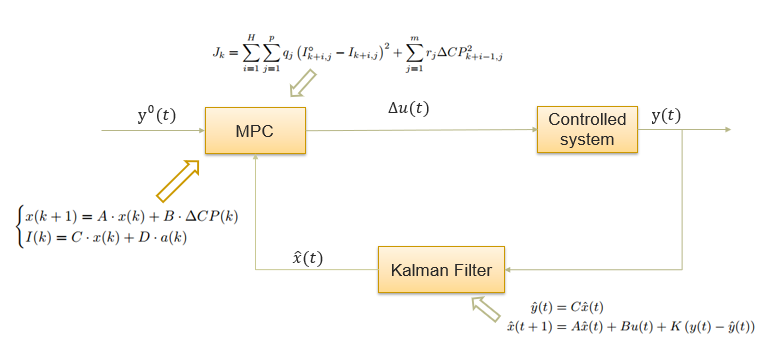
\includegraphics[width=\linewidth]{cobra}
	\caption{Control Scheme of CobRA}
\end{figure}

\section{Similarities}
Through the analysis of the two methods, we can get the similarities between them. 
\begin{itemize}
	\item They are both proactive latency-aware adaptation, making adaptation decisions with a look-ahead horizon and model the adaptation latency of the system.
	\item Adopt the MAPE-K framework. It involves \textit{monitoring}, \textit{analyzing}, \textit{planning} and \textit{executing} and share the \textit{knowledge}. 
	\item Use models to predict future behavior of the system. PLA constructs the system and environment to a whole MDP while CobRA uses a discrete-time linear dynamic system.
	\item Use receding horizon idea, which can make control more robust.
	\item Every adaptation period, they get a sequence of control actions, but only commiting to the first one.
\end{itemize}

Firstly, both of them adopt the idea of MPC, which is to use the prediction model to predict the future behavior of the system, and then use an optimization solution to make decisions. All of them adopt the idea of receding horizon, and get the decisions in the horizon at each decision-making moment, but only implement the first one, and make a new decision at the next decision-making moment according to the new measurements. While making adaptation decisions, the two methods take different methods. PLA solves the solution that maximizes the utility function, and CobRA solves the solution that minimizes the cost-function. They are two different constrained optimization problems. But the goal of both is same, which is to maximize the utility of the system. Therefore, under the same conditions, whether the two optimization problems can get the same solution is the first step to discuss the similarities between the two methods. We describe the two optimization problems and their constraints as follows:
\begin{itemize}
	\item {\verb|PLA|}:
	\begin{equation}
	\begin{aligned}
	&min\quad U=(s'+\Delta s)*cost-\dfrac{d'+\Delta d}{a}*(N-L), \\
	s.t.\quad &r\leq T,\\
	&-0.1\leq \Delta d\leq 0.1, -1\leq \Delta s\leq 1,\\
	&0\leq d'+\Delta d\leq 1,1\leq s'+\Delta s\leq 3
	\end{aligned}
	\end{equation}
	\item {\verb|CobRA|}:
	\begin{equation}
	\begin{aligned}
	&min\quad J=(r'-r^o)^2∗Q_{33}+(s'+\Delta s-s^o )^2∗Q_{11}\\
	&+(d'+\Delta d-d^o)^2∗Q_{22}+(\Delta s)^{2}∗R_{11}+(\Delta d)^2∗R_{22}\\
	s.t.\quad &-0.1\leq \Delta d\leq 0.1, -1\leq \Delta s\leq 1,\\
	&0\leq d'+\Delta d\leq 1,1\leq s'+\Delta s\leq 3
	\end{aligned}
	\end{equation}
\end{itemize}

When PLA obtains the optimal solution of its optimization problem in a certain state, that is, a decision is made, can MPC method make the same decision under this state? Is it possible to get the same solution for MPC constrained optimization? There are many factors we need to consider. First, PLA deals with discrete variables, while CobRA gets continuous control parameters, and for RUBiS system, we need to discretize the continuous variables to execute them, which may lead to non-optimal solution in the process of discretization. Secondly, PLA uses the predicted environment value in the calculation, while CobRA does not predict the future environment, and use the measured environment value in the solution. In CobRA, Kalman Filter is used to adjust the state of the system, which can feedback the changes of previous environment. Assuming that the number of servers in the current system is $s_0$, dimmer value is $d_0$, and the average arriving rate of requests is $a_0$, PLA solves the optimization problem and make the control decision. After the decision is implemented, the number of servers will be $s'$ and dimmer value will be $d'$. It is very important to set setpoints of CobRA's indicators. In order to get the same solution of CobRA, we naturally set setpoints to the target value calculated by PLA, that is, $s^o$ is set to $s'$ and $d^o$ is set to $d'$, but the target value of $r$ is open to discussion. However, the target value may not be satisfied, so weight values of cost function, that are $Q$ and $R$ matrixs, play important roles in decision making. When a reasonable weight value is designed and CobRA is optimized to get the same solution as PLA after discretization, it can be proved that the two methods can achieve the same control goal. But the circumstances are different. Does it make sense to talk about that?

\section{Differences}
By analyzing the design ideas of PLA  and CobRA, we can obtain some differences between them, which are mainly described in table \ref{tab:differences}.
\begin{table*}
	\caption{Differences between PLA and CobRA}
	\label{tab:differences}
	\begin{tabular}{ccl}
		%\newcommand{\tabincell}[2]{\begin{tabular}{@{}#1@{}}#2\end{tabular}}
		\toprule
		Features&PLA&CobRA\\
		\midrule
		Method & Architecture-based& Requirement-based\\
		Model for Environment & Predict and model to DTMC
		& Do not predict and regard as disturbance 
		\\
		Feedback & Open-loop
		 & Closed-loop\\
		Control  & tactics& Control parameter values
		\\
		Discrete or Continuous&discrete&Continuous\\
		Unsymmetric Latency&Model the unsymmetric latency&Can not model the unsymmetric latency
		\\
		Total Model&Non-linear MDP Model&Linear Dynamic Model\\
		Optimization&Utility function&System goals following boolean AND/OR semantics\\
		
		\bottomrule
	\end{tabular}
\end{table*}

First, while CobRA is requirement-based and uses cost function to describe requirements of the system, PLA is architecture-based and models the system as a MDP, thus it is suitable for discrete data. 
CobRA adopts the idea of control theory and to solve the optimization problem to get the incremental of control variables, which is more suitable for solving the problems with continuous variables. Also, one of the features of the RUBiS system is asymmetric latency, where adding servers has latency and the latency of reducing servers can be ignored.
PLA can clearly model the asymmetric delay, while the CobRA cannot model the asymmetric delay, and the traditional control field considers less on that. In CobRA's model, when the controller decides to remove a server, it will increase the dimmer to offset the delay.
In addition, when solving the optimization target, CobRA has constraints on variations of control paremeters in order to change them as small as possible, but there is no requirement for this in the PLA.
That's the same thing as, if we have multiple paths that can get maximum utility, We'll take the path that has the least change of control paremeters.

Two of the most significant differences are the way they model the environment and the ability of tolerancing uncertainties.
PLA considers the environment as the main uncertainty factor faced by the system. It deals with the future uncertainty factor within horizon by making a prediction to the possible changes of the future environment and modeling the environment as a DTMC.
CobRA considers the change of environment as disturbance of the system, and takes it as a feedforward signal. Through the feedback adjustment of Kalman Filter, the trend of environmental change can be gradually captured and the fluctuation of disturbance can be smoothed out.
As mentioned earlier, PLA is an open loop method, and the output in this decision period will not be used for calculation in the next decision period.
CobRA is a feedback method that uses the differences between the measured and calculated response times to dynamically adjust the state of the system at each decision point.

We mainly want to discuss the resolution and tolerance of these two kinds of uncertainty then we can obtain the advantages and disadvantages of the two methods. There are several perspectives. The most important one is whether it can achieve the goal and meet the requirements of adaptive control; and its ability to tolerate uncertain; and whether the implementation of this method requires high engineering cost. First of all, the resolution of the first kind of uncertainty reflects the realization of the adaptive controller function, that is, whether the controller can meet the control goal required by the designer.The second uncertainty determines the performance of the controller, which can be measured by saso properties. In GA's work\cite{plavscobra}, the realization of these two goals was discussed. Although there are many differences between these two methods, they can achieve similar control results. Through the comparative analysis of GAmoreno et al., we know that these two methods can achieve ideal control effect through fine tuning of parameters, but their tolerance to uncertainty and engineering cost are not discussed.

There are more factors need to consider. We focus on the tolerance effect of the two methods on the second uncertainty.
\subsection{Ideal Senorio}
First we need to define an ideal case, as the groundthruth to compare with other cases.
In an ideal situation, the system has no error in the prediction of the environment, the model of the system matches the actual system completely, and there is no error in the measurement. In this case, the system will make completely correct control decisions, that is, can keep getting the maximum utility.
As same to GA's work, to simulate the traffic generated by the users of the website, we used traces from the WorldCup ’98 trace archive\cite{worldcup}, and from the ClarkNet traces\cite{clarknet}. These traces represent a significant and realistic traffic\cite{traces}. We calculate the utility value of the system in the optimal case as for comparison.
Figure 2 shows the operation data statistics of the system under the ideal conditions. It can be found that the decision to add servers was made in advance in s because the load was predicted to increase in the future.
Under the load of WorldCup, the system can achieve the optimal utility of , and under the load of ClarkNet, the system can achieve the optimal utility of.
\subsection{Uncertainties from Environment}
\subsubsection{PLA}
The PLA use the prediction tool to predict the future environmental changes, and then constructs a probability tree model by taking the prediction errors into account using the EP-T three-point estimation method\cite{ept}. Since PLA's decision making mainly depends on the calculated response time, the predicted value of the environment is crucial in the adaptation decision process. If the prediction of the environment has non-negligible errors, the calculated response time will be greatly different from the real one, and if the threshold is triggered, PLA will make wrong decisions.\ref{fig:preenv}
\begin{figure}[h]
	\centering
	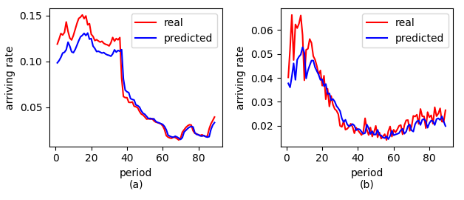
\includegraphics[width=\linewidth]{preenv}
	\caption{Prediction errors of workload.(a) for WorldCup,(b) for ClarkNet}
	
\end{figure}
We discuss the impact of the fluctuation of the two loads on the PLA's decision making. The load of WorldCup was relatively stable in the early stage, then increased sharply and decreased. The overall trend of ClarkNet load is of slow increase and then slow decrease, but fluctuations of arriving requests are quite frequent. In order to discuss the influence of the environment, we control other uncertainties to be certain, that is: the model matches the actual system, and the measurements are accurate. In this way, we assume that the system fully conforms to the calculated value of the queuing theory model, and the system only faces the prediction error of the environment as uncertainty factor.
此处应为对实验结果的分析
We use RPS toolkit to predict future environment, figure 1 describes the  actual environment and the estimated values of the two workloads.Figure \ref{fig:qncl}\ref{fig:qnwc} is indicators we care about the running system, which are the number of servers, the dimmer value and the average response time. It can be seen that under the WorldCup load, but not in s response time than the threshold decision making, because of environmental value, and according to the predicted environment response time is less than the threshold value calculation.
\begin{figure}[h]
	\centering
	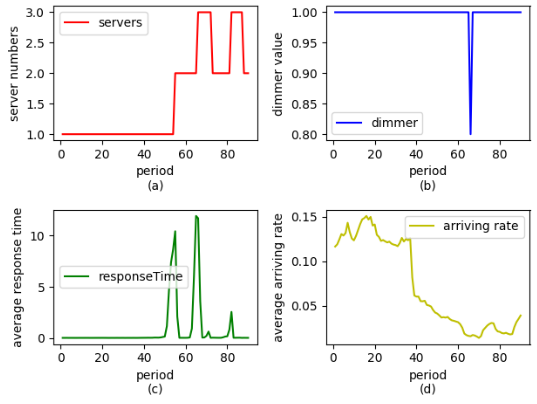
\includegraphics[width=\linewidth]{qnwc}
	\caption{Results of PLA under uncertain environment(WorldCup)}
	
\end{figure}
\begin{figure}[h]
	\centering
	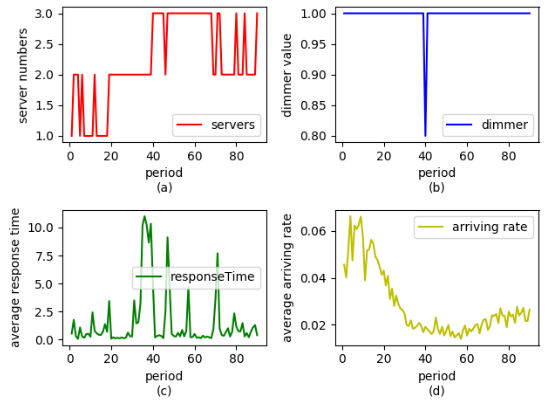
\includegraphics[width=\linewidth]{qncl}
	\caption{Results of PLA under uncertain environment(ClarkNet)}
	
\end{figure}
The decision is made in s, because the predicted value of the environment is, while the actual value is, the response time under the predicted value will exceed the threshold, while the actual value does not exceed the threshold.
What should be the conclusion?
How much lower would the earnings be under these two loads?
\subsubsection{CobRA}
Since CobRA adopts the idea of control theory and assumes that the system could be linearized near the equilibrium state, we can construct a simple linear model for the system. CobRA takes the environment as a disturbance of the system and uses it as a direct component to the model to affect the system's state. When we talk about the effect of the environment on the CobRA decision, we need the control model to be accurate. Here we assume that the system conforms to a linear model:
\begin{equation}
r=k_1*s+k_2*d+k_3*a
\end{equation}
We did this experiment with the same two workloads,\ref{fig:planokamlan}
\begin{figure}[h]
	\centering
	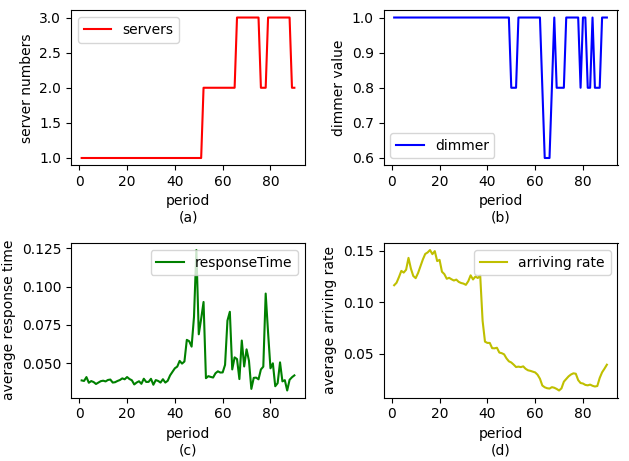
\includegraphics[width=\linewidth]{qkwc}
	\caption{Results of CobRA}
	
\end{figure}
此处应为对实验结果的分析
Statistics: in addition to the same as PLA, it also includes the state,
Analysis: timeout, adjustment, overadjustment discussion
\subsection{Uncertainties from Modeling}
\subsubsection{PLA}
PLA models the system and environment to a MDP. The system model only keeps track of the configuration information that is needed as input to the utility function including the number of active servers $s$, and the dimmer value $d$. This MDP model does not model the processing of each requests. To compute the average response time for every decision period according to the currunt system configuration and the environment, it uses a limited processor sharing (LPS) queueing theory model, due to each servers can only handle a limited number of requests simultaneously. However, the LPS queueing theory model has some limitations. The queuing theory model calculates the response time of a system in steady state. Accually, when there is an increase in workload that surpasses the current capacity of the system, a backlog of requests will build up. Until this backlog is worked off, returning to steady-state queue lengths, the observed response time is higher than normal, which lead to the computation error of the queuing model. For the RUBiS system, if the workload fluctuates more frequently, it is difficult to reach a steady state, even we only consider the average of a decision period.
\begin{figure}[h]
	\centering
	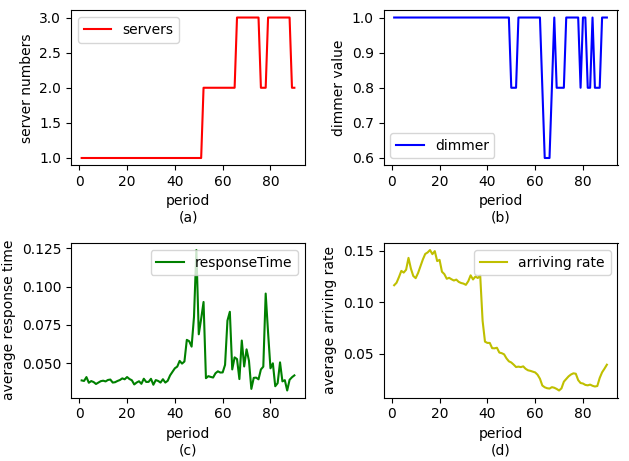
\includegraphics[width=\linewidth]{qkwc}
	\caption{Results of PLA without Feedback}

\end{figure}
此处应为对实验结果的分析
figure \ref{fig:qkwc} shows the results obtained with the PLA approach in the two workload. To discuss the influence of predicting model, we control the future environment is known. We can see that there are severe period where  the average response time is exceeding the threshold. That is due to the errors between predicted response time and the real one. At s, in this period, there has a sudden fluctuation of workload leading to a backup in servers, so the actual value is much higher than predicted.
\subsubsection{CobRA}
2) when the model is inaccurate
By using methods of system identification, we construct a linear model of the system and convert it into a state space equation, which can only describe a general trend of the system's behavior. Because our system is a complex nonlinear system, there inevitably exists a large error between the linear model and the actual system.
Analysis of experimental results:

Conclusion: although the CobRA model is very simple and crude, it can also achieve the control effect of consumption due to feedback regulation, and get a higher profit value.
此处应为对实验结果的分析
\subsubsection{PLA with Feedback}

The open-loop approach, such as PLA, relies heavily on model accuracy. MPC uses \textit{Kalman Filter} to achieve feedback adjustment that can gradually captures the trend of error, eliminates constant error and smooth out white noise. In this case,  we combine these two methods, using \textit{Kalman Filter} in PLA to adjust the estimated service rate to match the observations, and this deflated service rate will allow the predicction by queuing theory model better.
Researchers have proposed using Kalman Filter to estimate the value of system parameters at run time [50, 89, 146]. For RUBiS system, the average service time of each decision period is related to response time through LPS queuing model. Consequently, we can update the estimation of the service time, to minimize the error between predicted response time and the real one. In addition, using \textit{Kalman Filter} can also smooth characteristics that reduce jitter in the estimation.
\begin{figure}[h]
	\centering
	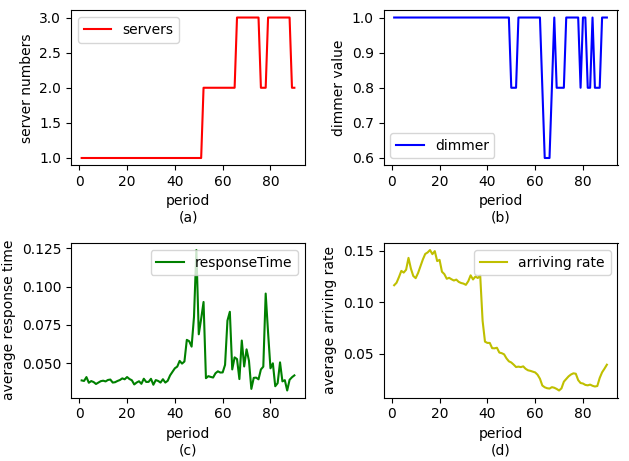
\includegraphics[width=\linewidth]{qkwc}
	\caption{Results of PLA with Feedback of WorldCup}
	
\end{figure}
此处应为对实验结果的分析
Figure \ref{fig:qkwc} shows the results of feedback-PLA. We can see that the response time are all below the threshold. And the utiltiy is much higher than without feedback.

\section{Related Work}
There are already several comparative evaluation works of self-adaptation approaches. The most relevant one is GA's work. They compared two proactive self-adaptation approaches, PLA and CobRA both in terms of development complexity, and of run-time performance. They found that two approaches have different dependencies and prerequisites for applying these approaches.
PLA requires the availability of theories and models for predicting specific types of property (e.g., queuing models to predict
performance), whereas CobRA does not require such models but demands some level of expertise of system dynamics and identification theory. CobRA is better suited to dealing with continuous control inputs, whereas PLA is better for discrete control. They suggested that a combined approach might lead to improved results over using either of the approaches in isolation.

In addition, other related works deals with comparation of reactive self-adaptation approaches. Reactive approaches do not  predict future system-environment behavior, and work well in settings in which adaptation latency is low and can be overlooked. They also can not make con-currunt control tactics. 
Angelopoulos et al. [35]compare architectural and requirement-centric models for adaptation and indicate combinations of features that might improve adaptation control. Shevtsov et al. [36] compare a control-based and an architecture-based approach to self-adaptation, reporting differences between them in performance and formal guarantees. Camara et al. compare code-based and architecture-based self-adaptation mechanisms, focusing on performance [37] and probabilistic guarantees on system resilience [38]. Camara et al. propose a framework for comparative evaluation of adaptive systems that focuses on resilience [40].

Although GA's work has made a systematic comparation between the two methods, in our work, we design a further analysis and get more conlusion by our experiments. We combine PLA with \textit{Kalman Filter} and explore its effects.
\section{Conclusion and Furture Work}

In this paper, based on GA's work, we analyzed and compared the two methods, PLA and CobRA, of proactive self-adaption. Firstly, we compared the design details of the two methods, and preliminarily got the similarities and differences between them.
In order to analyze the advantages and disadvantages of the two methods, we explored their tolerance to uncertainies and found that the simple open-loop method is sensitive to model errors and prediction errors and cannot solve problems such as constant errors and white noise.
PLA needs to be used when the model and the prediction of the environment are quite accurate.

Moreover, PLA will cost a lot of engineering cost in modeling.
However, if there are errors in the model and the environmental prediction, the method still cannot make the optimal decision. In this case, there is no need to spend a lot of money on modeling.
In the modeling phase of MPC method, it is considered that the system can be approximately linearized near the equilibrium state. So we can abstract the system to a simple linear model by tools such as system identification. 
Because MPC method has Kalman Filter feedback adjustment, it has good tolerance to error and guarantees of stability in control field.
In future work,
\bibliographystyle{ACM-Reference-Format}
\bibliography{acmart}
\end{document}
\endinput

